% !TEX root = ../../../main.tex
% 第二部分第四章第三节：Green 公式、Gauss 公式与 Stokes 公式
\section{Green 公式、Gauss 公式与 Stokes 公式}
\subsection*{区域与边界的方向}
\begin{definition}
不自交的闭曲线称为 Jordan 闭曲线。
\end{definition}
平面 Jordan 曲线定理指出：平面上的 Jordan 闭曲线将其补集分成两个互不相交的连通分支，其中一个有界，称为曲线的内部；另一个无界，称为曲线的外部。对 $\mathbb R^n$ 中的一条闭曲线，$n\ge3$ 时不存在这样的平面内外分割结论。

\begin{definition}
设 $D$ 为平面区域。如果 $D$ 内的任一闭曲线都可以不经过 $D$ 外的点而连续收缩为 $D$ 中一点，则称 $D$ 为单连通区域；否则称为复连通区域。
\end{definition}
\begin{definition}
沿区域边界行进时，区域始终在左侧的方向称为边界相对于区域的诱导定向，也称正向。对于有洞的区域，外边界取逆时针方向，内边界取顺时针方向。
\end{definition}

\par\addvspace{3pt}
{\centering
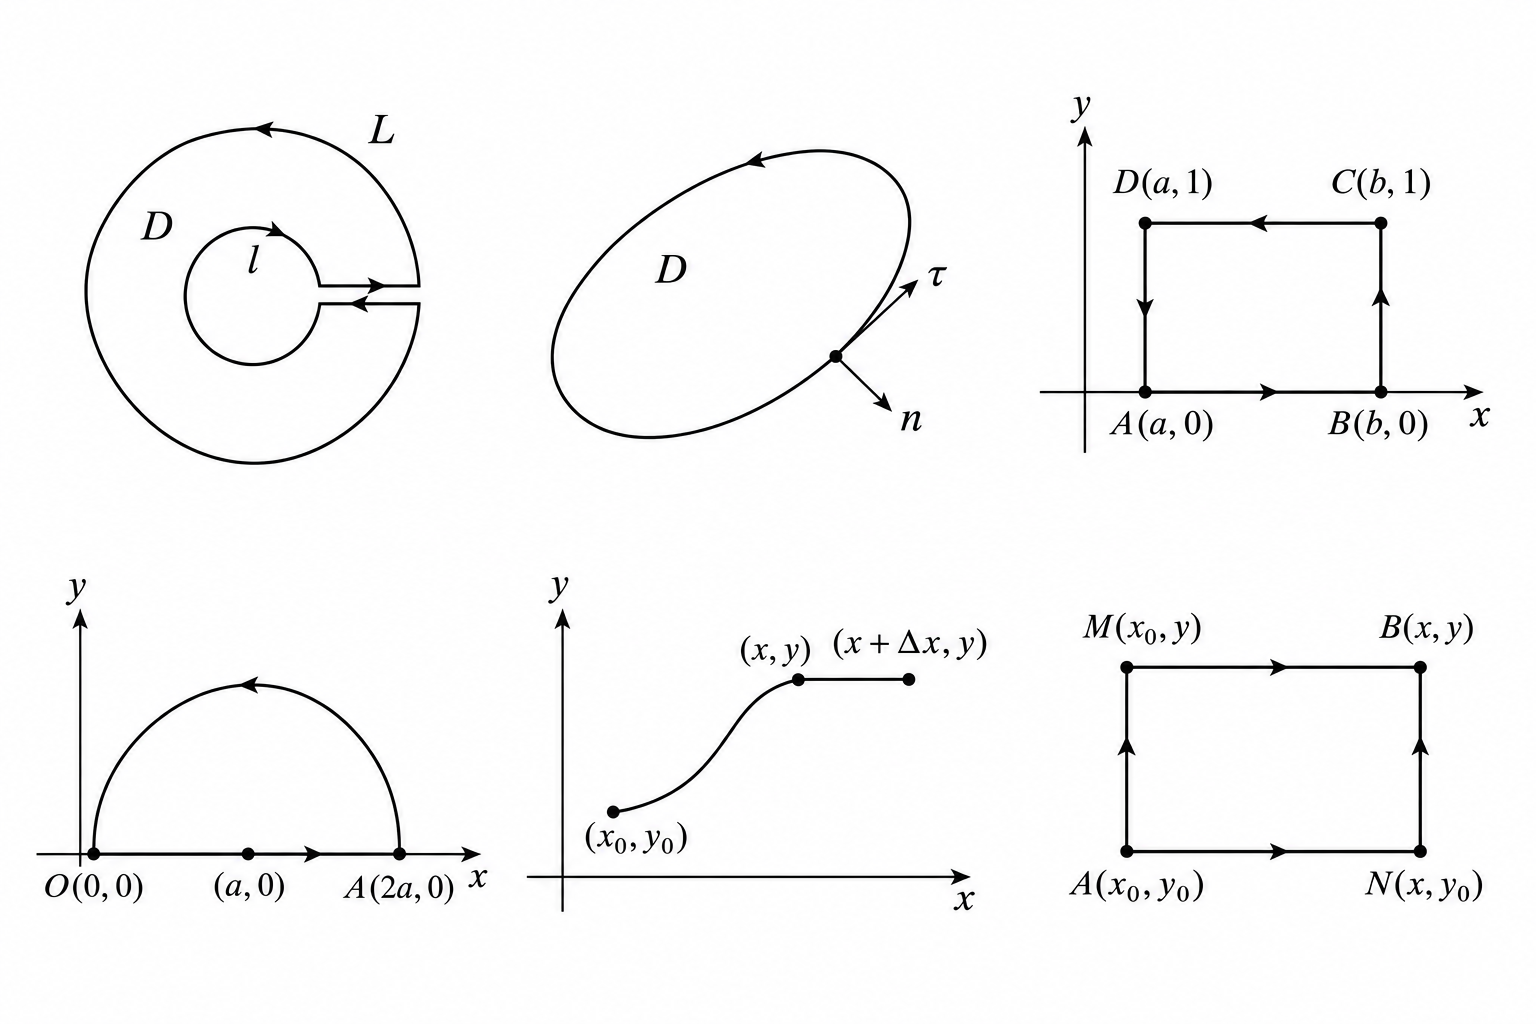
\includegraphics[width=0.2621\linewidth,viewport=77 551 429 917,clip]{figure/P2/green_diagrams_redrawn_hd.png}
\par}
\addvspace{3pt}
用连接内外边界的割线可把有洞区域切开。割线两岸的诱导方向相反，因此对应的曲线积分相互抵消；也可以先去掉宽度为 $\varepsilon$ 的窄条，再令 $\varepsilon\to0$。

\subsection*{Green 公式}
\begin{theorem}
设 $D$ 为平面有界单连通区域，边界 $\partial D$ 为分段光滑的简单闭曲线；$P,Q$ 在 $\overline D$ 的一个邻域内具有连续偏导数，则
\[
\oint_{\partial D}P\,\dd x+Q\,\dd y
=\displaystyle\iint_D\left(\frac{\partial Q}{\partial x}-\frac{\partial P}{\partial y}\right)\,\dd x\dd y,
\]
其中 $\partial D$ 取诱导定向，即逆时针方向。
\end{theorem}
\begin{proof}
先证明最简单的情形：$D$ 同时可表示为
\[
\begin{aligned}
D&=\{(x,y):a\le x\le b,\ y_1(x)\le y\le y_2(x)\}\\
&=\{(x,y):c\le y\le d,\ x_1(y)\le x\le x_2(y)\},
\end{aligned}
\]
其中边界函数分段光滑。由累次积分及 Newton--Leibniz 公式，
\begin{align*}
\displaystyle\iint_D Q_x\,\dd x\dd y
&=\int_c^d\dd y\int_{x_1(y)}^{x_2(y)}Q_x(x,y)\,\dd x\\
&=\int_c^d[Q(x_2(y),y)-Q(x_1(y),y)]\,\dd y.
\end{align*}
边界右侧由下向上，左侧由上向下，水平边上的 $\dd y=0$，所以
\[
\oint_{\partial D}Q\,\dd y
=\int_c^d Q(x_2(y),y)\,\dd y+\int_d^c Q(x_1(y),y)\,\dd y
=\displaystyle\iint_D Q_x\,\dd x\dd y.
\]
同样，
\[
\displaystyle\iint_D P_y\,\dd x\dd y
=\int_a^b[P(x,y_2(x))-P(x,y_1(x))]\,\dd x.
\]
边界下侧从左向右，上侧从右向左，竖直边上的 $\dd x=0$，因此
\[
\oint_{\partial D}P\,\dd x
=\int_a^bP(x,y_1(x))\,\dd x+\int_b^aP(x,y_2(x))\,\dd x
=-\displaystyle\iint_D P_y\,\dd x\dd y.
\]
相加即得所述公式。

若 $D$ 可有限分成上述类型的区域 $D_1,\ldots,D_N$，对每片分别使用公式并相加。每条内部公共边界恰出现两次且方向相反，故其积分抵消；余下的外边界恰为 $\partial D$。二重积分由区域可加性相加，得到 $D$ 上的公式。


% 按用户提供的局部引理、单位分解方法补全一般情形；展开坐标旋转和角点处理。
对一般分段光滑边界，下面用局部计算和单位分解补全证明。先说明所用概念。
\end{proof}


\begin{definition}
	设 $f$ 为开集 $U\subset\mathbb R^2$ 上的函数。称
	\[
	\operatorname{supp}f=\overline{\{p\in U:f(p)\ne0\}}^{\,U}
	\]
	为 $f$ 在 $U$ 中的支集，其中横线表示相对于 $U$ 的闭包。也就是说，支集由所有非零点及其在 $U$ 中的极限点组成；在支集之外，每一点都有一个邻域使 $f$ 恒为零。
	
	若 $\operatorname{supp}f$ 是包含于 $U$ 的紧集，则称 $f$ 在 $U$ 中具有紧支集。记 $K\Subset U$ 表示 $K$ 是包含于开集 $U$ 的紧集。此时 $K$ 与 $\mathbb R^2\setminus U$ 有正距离，因而紧支集函数在靠近 $U$ 外部的一带恒为零，可以在 $U$ 外延拓为零。
\end{definition}
\begin{lemma}[局部计算]
设 $V$ 是边界一点的局部邻域，在某个保持定向的正交坐标系中，$D\cap V$ 是一条 $C^1$ 图像曲线的一侧。若 $f\in C^1(V)$ 且 $\operatorname{supp}f\Subset V$，则将 $f$ 在 $V$ 外延拓为零后，有
\[
\oint_{\partial D} f\,\dd x
=-\displaystyle\iint_D f_y\,\dd x\dd y,
\qquad
\oint_{\partial D} f\,\dd y
=\displaystyle\iint_D f_x\,\dd x\dd y.
\]
若支集紧含于 $D$ 内，上述两式也成立，且等式两端均为零。
\end{lemma}
\begin{proof}
先设在原坐标中边界为 $y=\varphi(x)$，区域在其上方。因支集紧含于局部邻域，可以只在包含支集的有界矩形中积分，并在矩形外把函数记为零。于是
\begin{align*}
-\displaystyle\iint_D f_y\,\dd x\dd y
&=-\int\left[\int_{\varphi(x)}^{+\infty}f_y(x,y)\,\dd y\right]\,\dd x\\
&=\int f(x,\varphi(x))\,\dd x.
\end{align*}
这里无穷积分限只是简写，实际被积函数在有界范围外恒为零。区域在曲线上方时，正向边界从左向右，故右端就是 $\oint_{\partial D}f\,\dd x$。

为同时处理另一分量，令
\[
H(x)=\int_{\varphi(x)}^{+\infty} f(x,y)\,\dd y.
\]
由变限积分求导公式，
\[
H'(x)=\int_{\varphi(x)}^{+\infty}f_x(x,y)\,\dd y
-f(x,\varphi(x))\varphi'(x).
\]
$H$ 在一个有界区间外为零，所以 $\int H'(x)\,\dd x=0$，从而
\[
\displaystyle\iint_D f_x\,\dd x\dd y
=\int f(x,\varphi(x))\varphi'(x)\,\dd x
=\oint_{\partial D}f\,\dd y.
\]
若区域在曲线下方，则对 $y$ 的积分从 $-\infty$ 到 $\varphi(x)$，正向边界也改为从右向左。两处符号相应改变，所得两式不变。

现在说明旋转坐标的情形。上面两式对任意紧支集向量场 $\boldsymbol A=(A_1,A_2)$ 相加，等价于局部的通量等式
\[
\oint_{\partial D}\boldsymbol A\cdot\boldsymbol n\,\dd s
=\displaystyle\iint_D(\partial_xA_1+\partial_yA_2)\,\dd x\dd y.
\]
作保持定向的正交变换 $p=R\widetilde p+b$，令 $\widetilde{\boldsymbol A}(\widetilde p)=R^{\mathsf T}\boldsymbol A(R\widetilde p+b)$。正交变换保持长度、面积和内积，单位外法向量按同一矩阵变换，且由链式法则
\[
D\widetilde{\boldsymbol A}=R^{\mathsf T}(D\boldsymbol A)R,
\quad
\partial_{\widetilde x}\widetilde A_1+\partial_{\widetilde y}\widetilde A_2
=\partial_xA_1+\partial_yA_2.
\]
其中 $D\boldsymbol A$ 是向量场的导数矩阵，后一等式可由 $RR^{\mathsf T}=I$ 直接展开得到。因此通量等式不因旋转改变。分别取 $\boldsymbol A=(0,-f)$ 和 $(f,0)$，再用 $\boldsymbol n\,\dd s=(\dd y,-\dd x)$，就得到原坐标中的两条结论。

若支集紧含于 $D$，边界积分为零；在包含支集的矩形中先对相应变量积分，利用矩形边上 $f=0$，两个偏导数的面积积分也均为零。
\end{proof}

\begin{definition}
设紧集 $K$ 被有限个开集 $V_1,\ldots,V_N$ 覆盖。若光滑非负函数 $\rho_1,\ldots,\rho_N$ 在 $K$ 的某个邻域内满足
\[
\sum_{i=1}^N\rho_i=1,\qquad \operatorname{supp}\rho_i\Subset V_i,
\]
则称这些函数构成从属于该覆盖的光滑单位分解。它把一个函数分成各自只在一个局部邻域内起作用的有限个函数。
\end{definition}
这样的单位分解可以构造如下。对每个 $p\in K$ 取小球，使其二倍球的闭包仍在某个 $V_i$ 中；由紧性选出有限个小球覆盖 $K$。在每个二倍球中取光滑非负函数 $\eta_j$，使它在对应小球上严格为正，在二倍球外为零。例如，平移缩放后可用
\[
\eta(p)=
\begin{cases}
\exp\bigl(-1/(1-|p|^2)\bigr),&|p|<1,\\
0,&|p|\ge1.
\end{cases}
\]
令 $h=\sum_j\eta_j$，则 $h>0$ 于 $K$ 的一个邻域。再取光滑函数 $\chi$，使它在 $K$ 附近等于 $1$，且支集紧含于 $\{h>0\}$：可取充分小的 $c>0$ 使 $h>2c$ 于 $K$，再令 $\chi=\psi(h)$，其中光滑函数 $\psi$ 在 $[0,c]$ 为零，在 $[2c,+\infty)$ 为 $1$。于是 $\chi\eta_j/h$ 在 $h>0$ 处定义、其余处置零，便得到所需函数；把属于同一 $V_i$ 的项相加即得 $\rho_i$。

\begin{proof}[Green 公式一般情形的证明]
先设 $P,Q$ 在所有角点附近为零。它们的支集与 $\overline D$ 的交集是紧集，且避开有限个角点。在光滑边界点处，由正则性及隐函数定理，可以选取保持定向的正交坐标，使边界局部成为 $C^1$ 图像。用这些边界邻域和完全位于 $D$ 内的邻域覆盖该紧集，取有限子覆盖及相应单位分解。

令 $P_i=\rho_iP$、$Q_i=\rho_iQ$，则在 $\overline D$ 上有
\[
P=\sum_iP_i,\qquad Q=\sum_iQ_i,
\qquad P_y=\sum_i(P_i)_y,\qquad Q_x=\sum_i(Q_i)_x.
\]
对每一项用局部引理；支集在内部的项两端均为零。逐项相加，得到
\begin{align*}
\oint_{\partial D}P\,\dd x+Q\,\dd y
&=\sum_i\oint_{\partial D}(P_i\,\dd x+Q_i\,\dd y)\\
&=\sum_i\displaystyle\iint_D[(Q_i)_x-(P_i)_y]\,\dd x\dd y\\
&=\displaystyle\iint_D(Q_x-P_y)\,\dd x\dd y.
\end{align*}

最后去掉在角点附近为零的限制。记角点为 $c_1,\ldots,c_m$。取光滑截断函数 $\theta_\varepsilon$，使它在每个 $B(c_j,\varepsilon)$ 内为零，在所有 $B(c_j,2\varepsilon)$ 外为 $1$，且
\[
0\le\theta_\varepsilon\le1,\qquad
|\nabla\theta_\varepsilon|\le C/\varepsilon.
\]
这里 $B(c,r)$ 为以 $c$ 为中心、半径为 $r$ 的开圆盘，$\nabla\theta=(\theta_x,\theta_y)$。可将固定光滑径向截断函数缩放后取有限个因子的乘积得到上述函数。

对 $P_\varepsilon=\theta_\varepsilon P$、$Q_\varepsilon=\theta_\varepsilon Q$ 使用已经证明的公式。它们与原函数的差只出现在角点的 $2\varepsilon$ 邻域内。这些邻域的总面积为 $O(\varepsilon^2)$；正则 $C^1$ 边界弧在其中的总长度为 $O(\varepsilon)$，因为弧在角点每一侧均可表示为导数有界的局部图像。$P,Q$ 及其一阶偏导数在 $\overline D$ 附近有界，所以边界积分之差为 $O(\varepsilon)$。

另一方面，
\[
(Q_\varepsilon)_x-(P_\varepsilon)_y
=\theta_\varepsilon(Q_x-P_y)
+(\theta_\varepsilon)_xQ-(\theta_\varepsilon)_yP.
\]
第一项与 $Q_x-P_y$ 的面积积分之差为 $O(\varepsilon^2)$；后两项的积分绝对值不超过常数乘以 $\varepsilon^{-1}\varepsilon^2$，因而为 $O(\varepsilon)$。令 $\varepsilon\to0$，就得到原来的 $P,Q$ 所满足的 Green 公式。一般分段光滑边界的证明完成。
\end{proof}

Green 公式也适用于边界由有限条互不相交的分段光滑 Jordan 曲线组成的有洞区域。以一个洞为例，外边界记为 $L$，内边界记为 $l$，取割线 $MN$ 后，割线两岸的积分抵消，故
\[
\begin{aligned}
\displaystyle\iint_D(Q_x-P_y)\,\dd x\dd y
&=\left(\int_L+\int_{MN}+\int_l+\int_{NM}\right)(P\,\dd x+Q\,\dd y)\\
&=\left(\int_L+\int_l\right)(P\,\dd x+Q\,\dd y)
=\oint_{\partial D}P\,\dd x+Q\,\dd y.
\end{aligned}
\]
这里 $L$ 逆时针、$l$ 顺时针，与区域的诱导定向一致。

\subsection*{Green 公式的几种应用}
\begin{enumerate}
\item 记正向边界的单位切向量为 $\boldsymbol\tau$，单位外法向量为 $\boldsymbol n$。若 $\boldsymbol\tau=(\tau_x,\tau_y)$，则 $\boldsymbol n=(\tau_y,-\tau_x)$，故
\[
\cos(\vect n,y)=-\cos(\vect \tau,x),\qquad \cos(\vect n,x)=\sin(\vect \tau,x),
\]
其中后一式把切向角理解为有向角。令 $P=-G,Q=F$，得到
\begin{align*}
\displaystyle\iint_D(F_x+G_y)\,\dd x\dd y
&=\oint_{\partial D}F\,\dd y-G\,\dd x\\
&=\oint_{\partial D}[F\cos(\vect n,x)+G\cos(\vect n,y)]\,\dd s.
\end{align*}
\par\addvspace{3pt}
{\centering
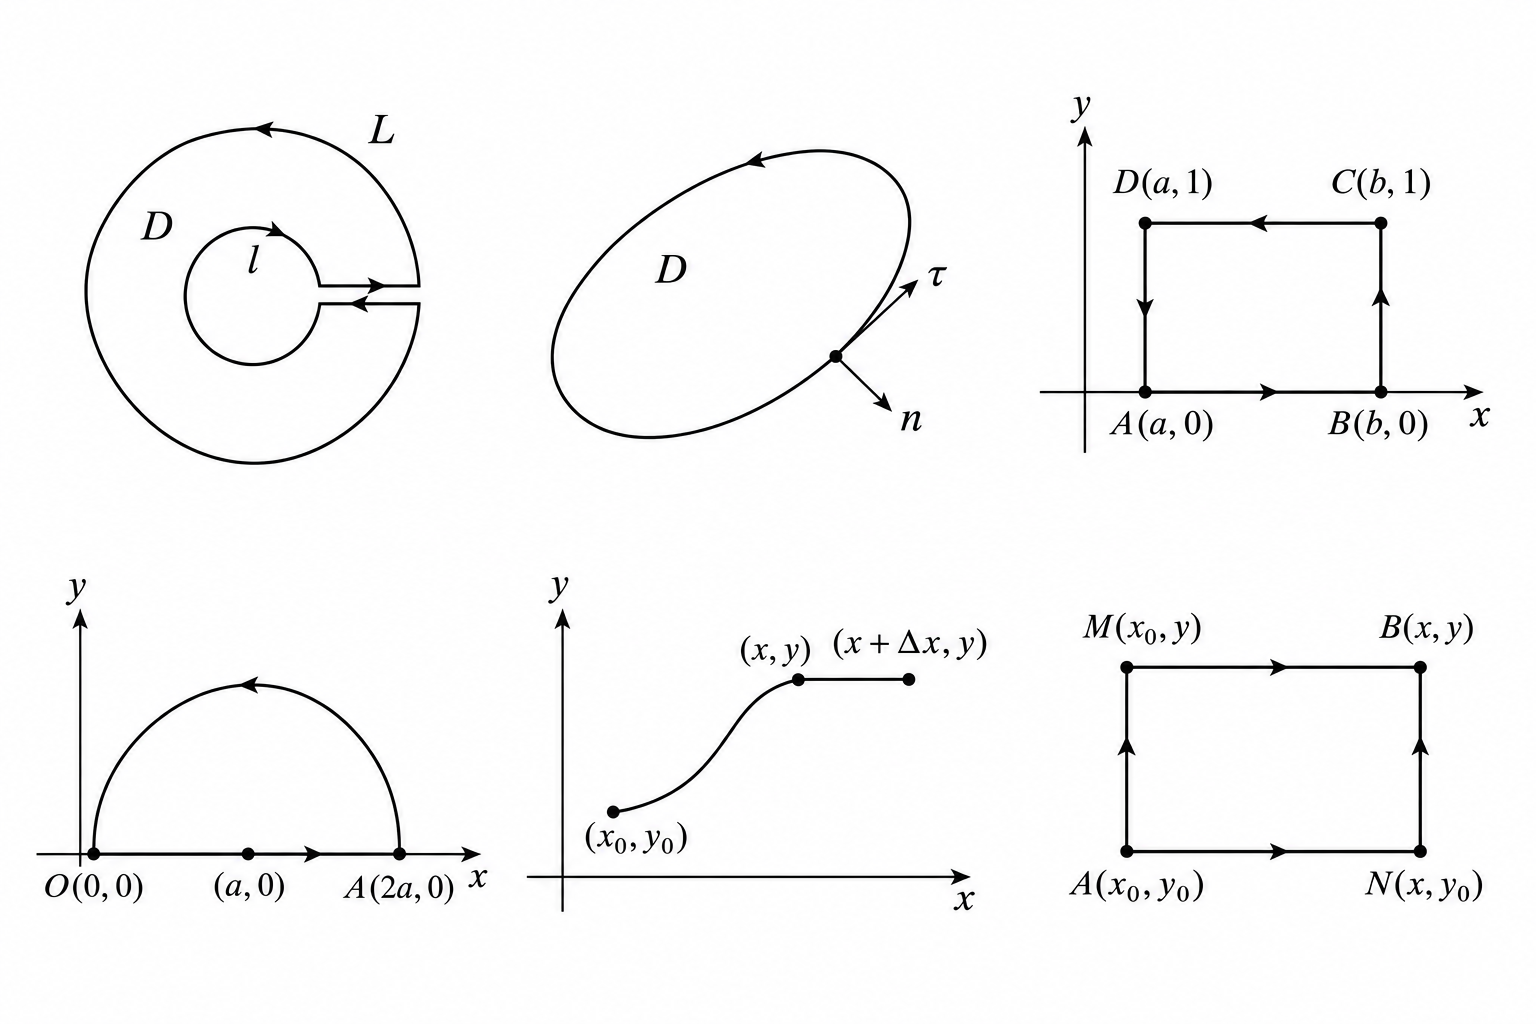
\includegraphics[width=0.2884\linewidth,viewport=543 577 955 883,clip]{figure/P2/green_diagrams_redrawn_hd.png}
\par}
\addvspace{3pt}
\item Green 公式推广了 Newton--Leibniz 公式。设 $f\in C^1([a,b])$，在 $D=[a,b]\times[0,1]$ 上取 $P=0,Q=f(x)$，则
\[
\displaystyle\iint_Df'(x)\,\dd x\dd y=\oint_{\partial D}f(x)\,\dd y.
\]
\par\addvspace{3pt}
{\centering
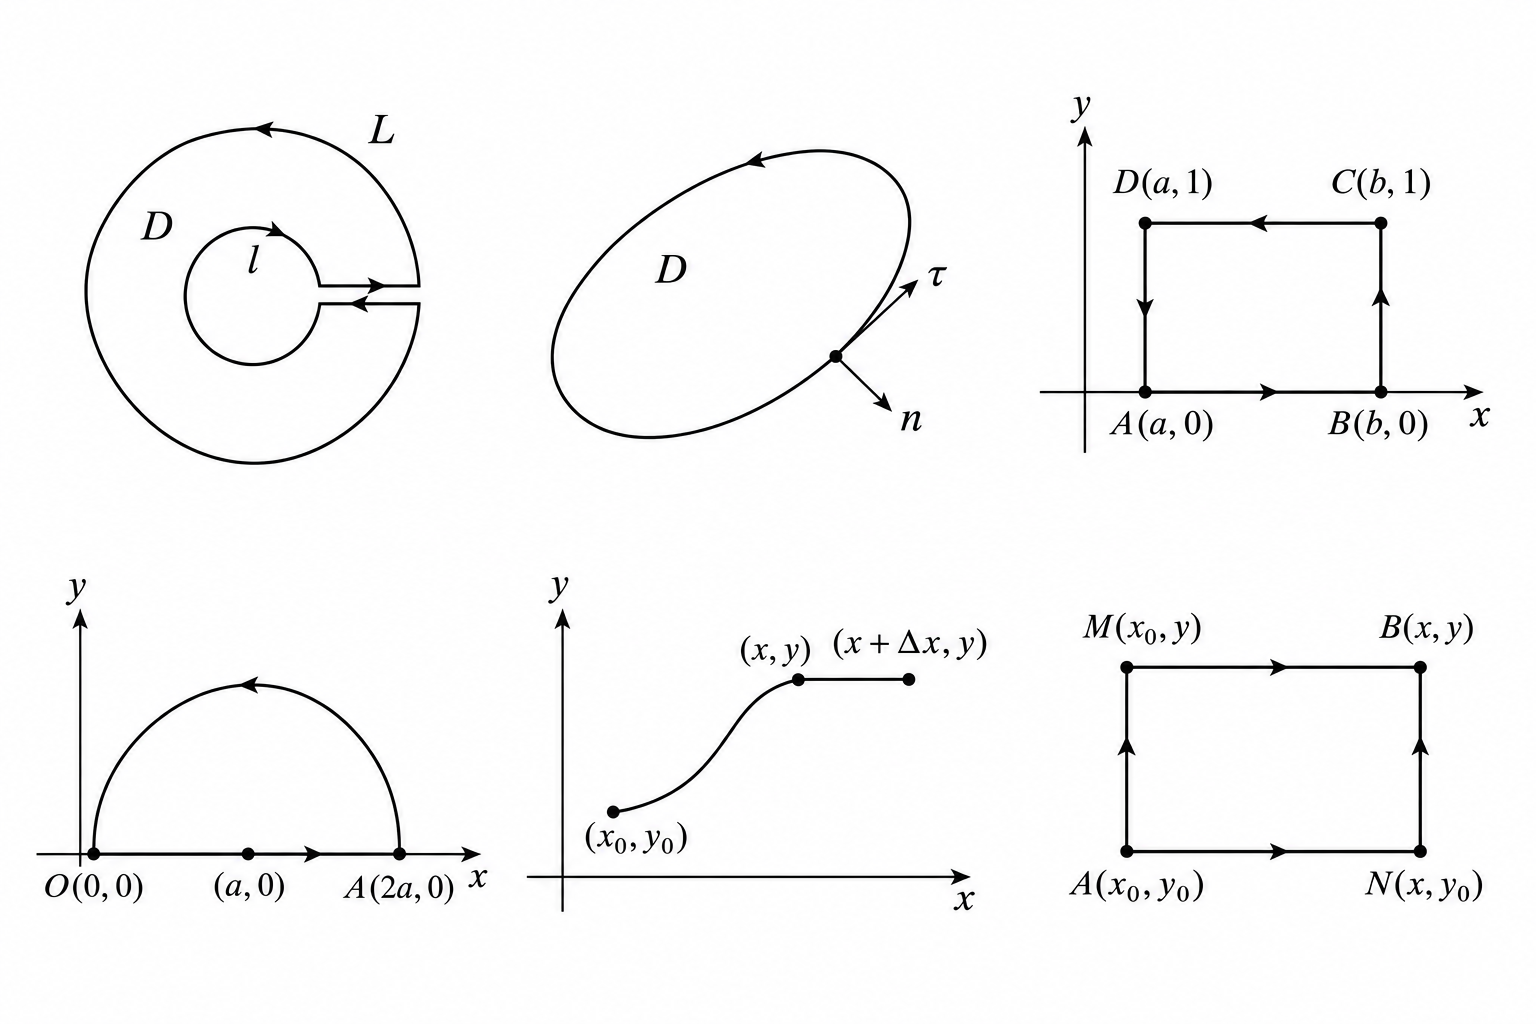
\includegraphics[width=0.45\linewidth,viewport=1032 563 1498 935,clip]{figure/P2/green_diagrams_redrawn_hd.png}
\par}
\addvspace{3pt}
左端等于 $\displaystyle\int_a^bf'(x)\,\dd x$。右端的两条水平边贡献为零，右侧竖边向上，左侧竖边向下，因而
\[
\oint_{\partial D}f(x)\,\dd y=\int_0^1 f(b)\,\dd y+\int_1^0 f(a)\,\dd y=f(b)-f(a).
\]
于是 $\displaystyle\int_a^bf'(x)\,\dd x=f(b)-f(a)$。
\item 若 $D$ 的边界为分段光滑简单闭曲线，面积为 $S$，则
\[
S=\displaystyle\iint_D1\,\dd x\dd y
=\oint_{\partial D}x\,\dd y
=-\oint_{\partial D}y\,\dd x
=\frac12\oint_{\partial D}(x\,\dd y-y\,\dd x).
\]
\end{enumerate}
% 原文面积公式的证明留给读者。
\begin{proof}
在 Green 公式中依次取 $(P,Q)=(0,x)$、$(-y,0)$ 和 $(-y/2,x/2)$，三次均有 $Q_x-P_y=1$，故分别得到三条边界积分公式。
\end{proof}

\begin{example}
计算
\[
I=\int_L(e^x\sin y-my)\,\dd x+(e^x\cos y-m)\,\dd y,
\]
其中 $L$ 为圆 $(x-a)^2+y^2=a^2$（$a>0$）的上半圆周，方向从 $A(2a,0)$ 到 $O(0,0)$。
\end{example}
\begin{solution}
$L$ 不是闭曲线，补入从 $O$ 到 $A$ 的直线段 $\overrightarrow{OA}$，得到上半圆域 $D$ 的正向边界。
\par\addvspace{3pt}
{\centering
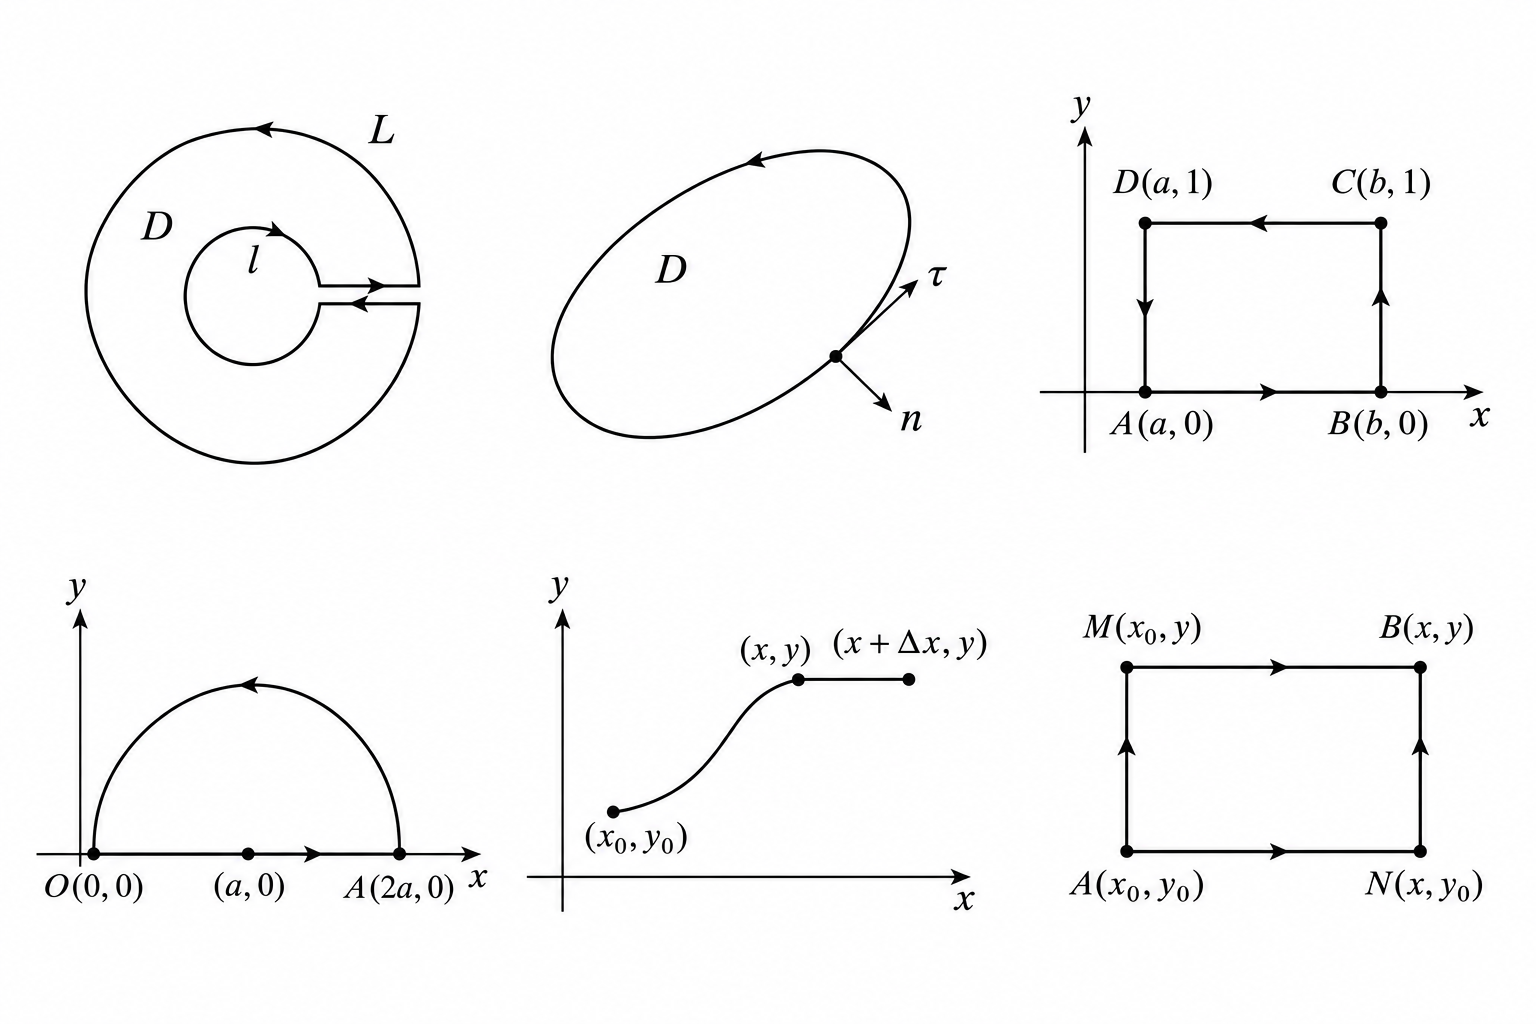
\includegraphics[width=0.5126\linewidth,viewport=29 112 495 453,clip]{figure/P2/green_diagrams_redrawn_hd.png}
\par}
\addvspace{3pt}
取 $P=e^x\sin y-my$、$Q=e^x\cos y-m$，则
\[
P_y=e^x\cos y-m,\qquad Q_x=e^x\cos y.
\]
由 Green 公式，
\[
I+\int_{\overrightarrow{OA}}P\,\dd x+Q\,\dd y
=m\displaystyle\iint_D1\,\dd x\dd y=\frac{m\pi a^2}{2}.
\]
沿 $\overrightarrow{OA}$，$y=0$、$\dd y=0$、$P(x,0)=0$，故补线积分为零。因此
\[
I=\frac{m\pi a^2}{2}.
\]
\end{solution}

\subsection*{曲线积分与路径无关}
\begin{definition}
设 $D$ 为平面区域，$P,Q$ 在 $D$ 上连续。若对任意 $A,B\in D$，曲线积分 $\int_LP\,\dd x+Q\,\dd y$ 只与端点 $A,B$ 有关，与 $D$ 内连接它们的分段光滑路径 $L$ 无关，则称该曲线积分与路径无关；否则称为与路径有关。
\end{definition}
\begin{theorem}[Green 定理]
(Green 定理)设 $D$ 为平面单连通区域，$P,Q\in C^1(D)$。以下四个命题等价：
\begin{enumerate}
\item 对 $D$ 内任意分段光滑闭曲线 $L$，有 $\displaystyle\oint_LP\,\dd x+Q\,\dd y=0$；
\item 曲线积分 $\displaystyle\int_LP\,\dd x+Q\,\dd y$ 与路径无关；
\item 存在 $D$ 上的可微函数 $U$，使 $\dd U=P\,\dd x+Q\,\dd y$；
\item 在 $D$ 内 $P_y=Q_x$。
\end{enumerate}
其中第三条称 $P\,\dd x+Q\,\dd y$ 为 $U$ 的全微分，并称 $U$ 为该 $1$-形式的原函数。
\end{theorem}
\begin{proof}
\begin{enumerate}
\item[$(1)\Rightarrow(2)$] 取任意从 $A$ 到 $B$ 的两条路径 $L_1,L_2$，闭曲线 $C=L_1+(-L_2)$ 满足
\[
0=\oint_C P\,\dd x+Q\,\dd y
=\int_{L_1}P\,\dd x+Q\,\dd y-\int_{L_2}P\,\dd x+Q\,\dd y.
\]
故两条路径的积分相等。
\item[$(2)\Rightarrow(3)$] 固定 $(x_0,y_0)\in D$，定义
\[
U(x,y)=\int_{(x_0,y_0)}^{(x,y)}P\,\dd x+Q\,\dd y.
\]
区域内两点可用分段光滑路径连接，路径无关性保证定义唯一。由于 $D$ 开，在 $(x,y)$ 附近的一小段水平线仍位于 $D$ 内，于是
\[
\frac{U(x+\Delta x,y)-U(x,y)}{\Delta x}
=\frac1{\Delta x}\int_x^{x+\Delta x}P(t,y)\,\dd t\longrightarrow P(x,y).
\]
\par\addvspace{3pt}
{\centering
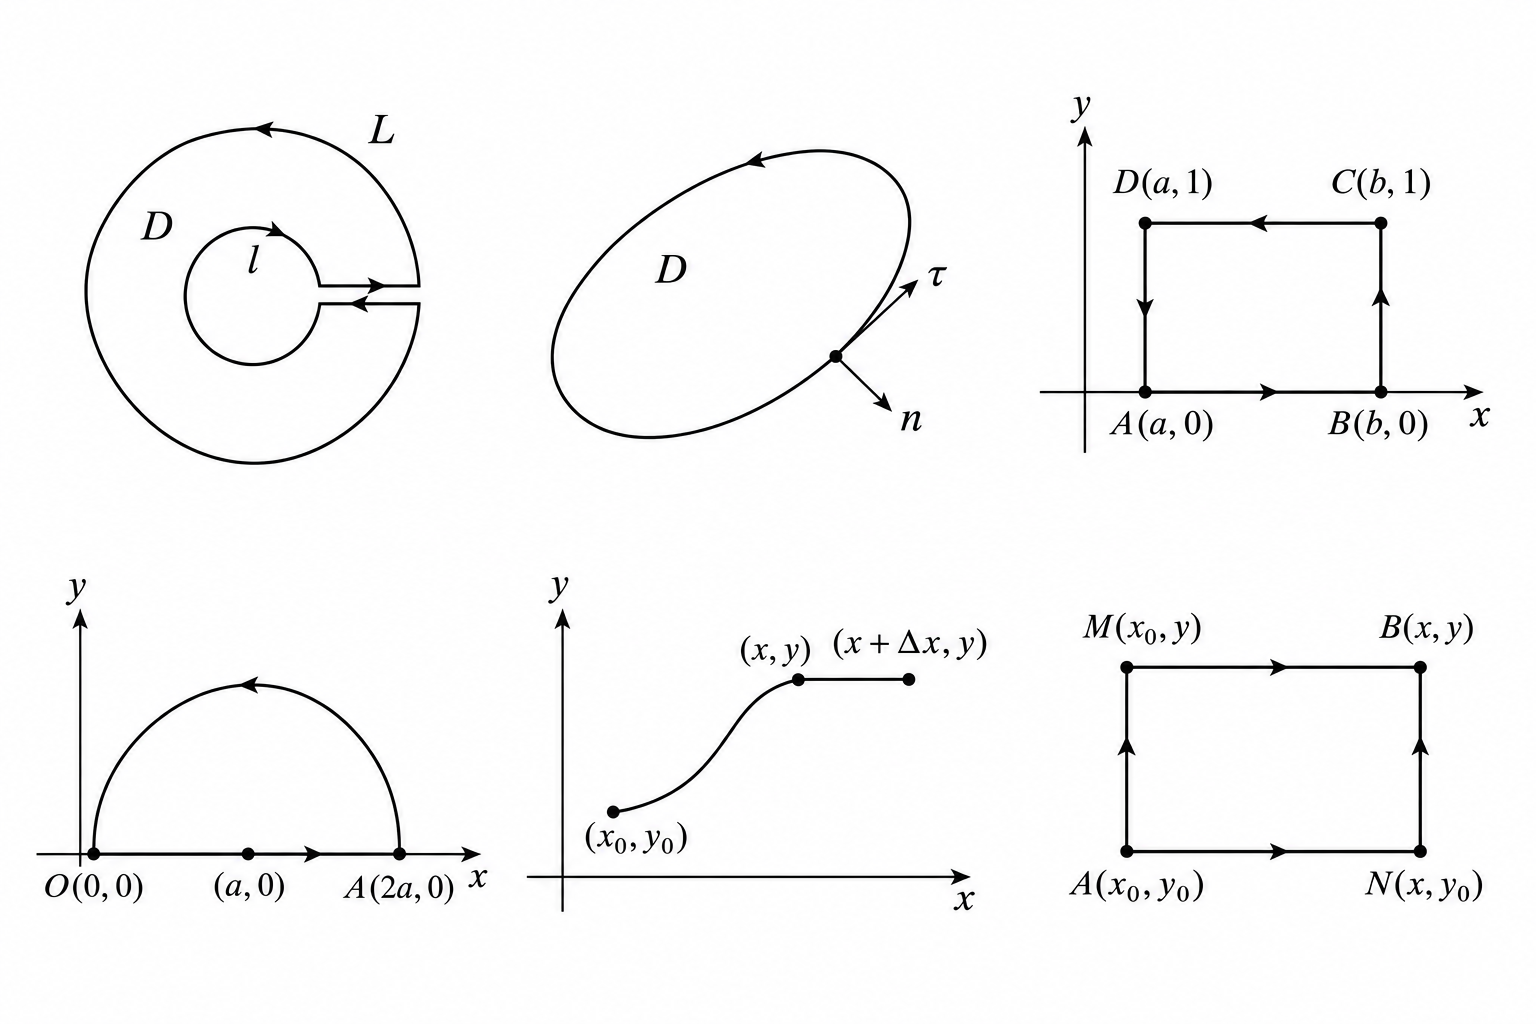
\includegraphics[width=0.45\linewidth,viewport=519 104 994 455,clip]{figure/P2/green_diagrams_redrawn_hd.png}
\par}
\addvspace{3pt}
沿竖直短线段同理得 $U_y=Q$。因 $P,Q$ 连续，$U$ 可微，且 $\dd U=P\,\dd x+Q\,\dd y$。
\item[$(3)\Rightarrow(4)$] 由 $U_x=P,U_y=Q$ 及 $P,Q\in C^1(D)$，可知 $U\in C^2(D)$。混合偏导数相等，故
\[
P_y=U_{xy}=U_{yx}=Q_x.
\]
\item[$(4)\Rightarrow(1)$] 先设 $L$ 为简单闭曲线。单连通性保证其围成的内部 $\widetilde D$ 仍在 $D$ 中，由 Green 公式，
\[
\oint_LP\,\dd x+Q\,\dd y
=\pm\displaystyle\iint_{\widetilde D}(Q_x-P_y)\,\dd x\dd y=0.
\]
% 以下补足原图从简单闭曲线到一般闭路径的适用范围。
若 $L$ 是一般分段光滑闭路径，先对有限自交的闭折线按交点分解成有限条简单闭折线；每条积分均为零，相加仍为零。再在 $D$ 内用闭折线逼近 $L$：在每段 $C^1$ 参数区间上取足够细的划分并连接相邻点。由于路径像为 $D$ 内的紧集，细划分的弦段仍在 $D$ 内；由参数导数的一致连续性，折线的分段导数在各光滑段上一致逼近原导数，位置也一致逼近原路径。因此 $P,Q$ 的连续性保证折线积分趋于 $L$ 上的积分。若折线有退化重合边，可作任意小顶点扰动使交点有限，积分随扰动连续变化，结论仍成立。故一般闭路径的积分也为零。
\end{enumerate}
\end{proof}

\begin{theorem}
设 $D$ 为平面单连通区域，$P,Q$ 在 $D$ 上连续。曲线积分与路径无关的充分必要条件是 $P\,\dd x+Q\,\dd y$ 在 $D$ 上存在原函数 $U$。此时对于任意从 $A(x_A,y_A)$ 到 $B(x_B,y_B)$ 的分段光滑路径，有
\[
\int_A^B P\,\dd x+Q\,\dd y=U(x_B,y_B)-U(x_A,y_A).
\]
\end{theorem}
\begin{proof}
若积分与路径无关，按前一定理的构造定义 $U$；该构造只需 $P,Q$ 连续，就有 $U_x=P,U_y=Q$。取一条从基点到 $A$ 的路径 $l$，再接上从 $A$ 到 $B$ 的路径 $L$，则
\[
U(A)=\int_lP\,\dd x+Q\,\dd y,\qquad
U(B)=\int_{l+L}P\,\dd x+Q\,\dd y.
\]
相减即得积分等于 $U(B)-U(A)$。

反之，若存在原函数 $U$，沿光滑路径 $L:(x(t),y(t))$，$a\le t\le b$，由链式法则，
\begin{align*}
\int_LP\,\dd x+Q\,\dd y
&=\int_a^b[P(x(t),y(t))x'(t)+Q(x(t),y(t))y'(t)]\,\dd t\\
&=\int_a^b\frac{\dd}{\dd t}U(x(t),y(t))\,\dd t
=U(B)-U(A).
\end{align*}
分段光滑路径逐段使用此式，中间端点值抵消，结论相同。因此积分与路径无关。
\end{proof}

求原函数常用两条折线路径。固定基点 $A=(x_0,y_0)$，令 $B=(x,y)$，$N=(x,y_0)$、$M=(x_0,y)$。
\par\addvspace{3pt}
{\centering
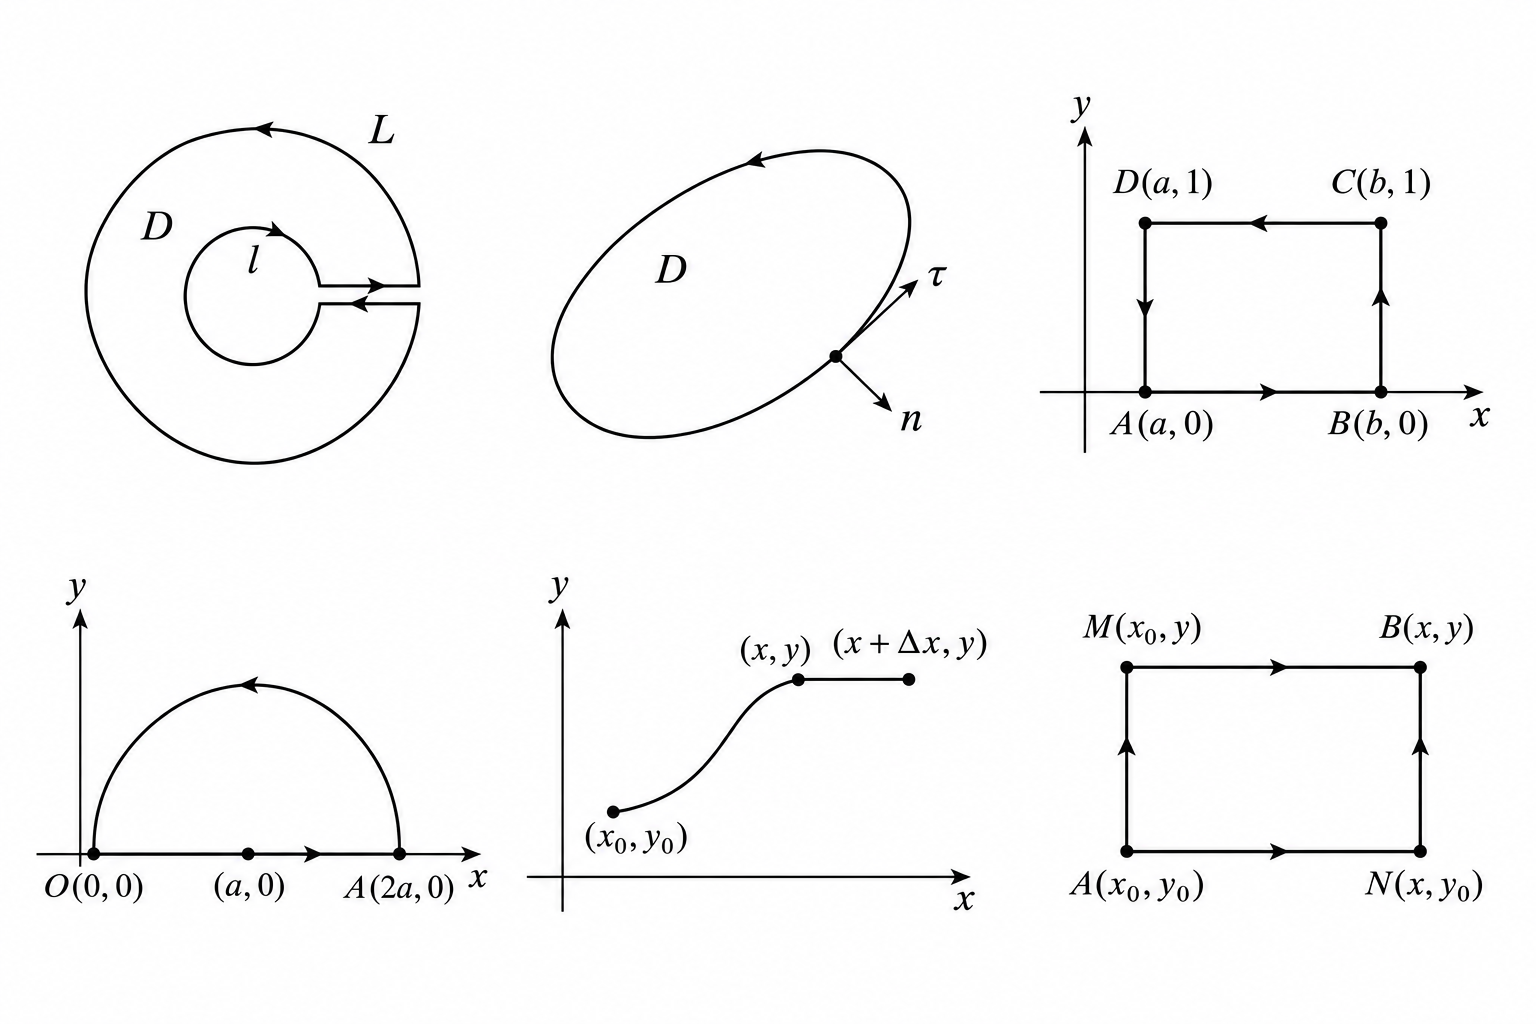
\includegraphics[width=0.4\linewidth,viewport=1062 114 1490 419,clip]{figure/P2/green_diagrams_redrawn_hd.png}
\par}
\addvspace{3pt}
当所用折线全部位于 $D$ 内时，沿 $ANB$ 积分得到
\[
U(x,y)=\int_{x_0}^x P(t,y_0)\,\dd t+\int_{y_0}^y Q(x,s)\,\dd s+c.
\]
沿 $AMB$ 则得到
\[
U(x,y)=\int_{y_0}^y Q(x_0,s)\,\dd s+\int_{x_0}^x P(t,y_0)\,\dd t+c,
\qquad c=U(x_0,y_0).
\]
